\documentclass[12pt,addpoints,answers]{repaso}
\grado{1}
\nivel{Secundaria}
\cicloescolar{2024-2025}
\materia{Matemáticas 1 \normalfont \color{darkgray} \\[-0.2em] \small con adecuación curricular a Matemáticas 5$^\circ$ de Primaria}
\unidad{1, 2 y 3}
\title{Practica la Unidad}
\aprendizajes{\scriptsize%
	% \item Estudio de los números.
\item Ordena, lee, escribe e identifica regularidades en números naturales de hasta nueve cifras. Lee, escribe y ordena números decimales hasta diezmilésimos en notación decimal y letra, y los interpreta en diferentes contextos.
	% \item Suma y resta, su relación como operaciones inversas.
	\item Propone y resuelve situaciones problemáticas que implican sumas y restas con números decimales utilizando el algoritmo convencional y fracciones con diferentes denominadores. 
	% \item Multiplicación y división, su relación como operaciones inversas.
	\item Resuelve situaciones problemáticas vinculadas a diferentes contextos que implican multiplicar números fraccionarios y números decimales, con un número natural como multiplicador.También, dividir números naturales y el cociente resulte un número decimal.
	% \item Relaciones de proporcionalidad.
	\item Resuelve situaciones problemáticas de proporcionalidad en las que determina valores faltantes de números naturales, a partir de diferentes estrategias (cálculo del valor unitario, de dobles, triples o mitades).
	% \item Ubicación espacial.
	\item Elabora e interpreta croquis para comunicar la ubicación de seres vivos, objetos, trayectos o lugares.
	% \item Medición de la longitud, masa y capacidad.
	% \item Figuras y cuerpos geométricos y sus características.
	\item Reconoce y describe semejanzas y diferencias entre un prisma y una pirámide; propone desarrollos planos para construir prismas rectos cuadrangulares o rectangulares.
	% \item Perímetro, área y noción de volumen.
	\item Calcula el perímetro y área de diferentes polígonos. Construye y usa fórmulas para calcular el perímetro de cualquier polígono, a partir de sumar la longitud de todos sus lados o multiplicar el número de lados por la medida de uno de ellos.
	% \item Organización e interpretación de datos.
	\item Construye tablas y gráficas de barras, e interpreta información cuantitativa y cualitativa contenida en ellas.
	% \item Nociones de probabilidad. 
	\item Identifica situaciones de distintos contextos en las que interviene o no el azar; registra resultados de experiencias aleatorias en tablas de frecuencias y expresa la frecuencia absoluta y la relativa.
	  }
\author{Melchor Pinto, JC}
\begin{document}
\INFO
\begin{multicols}{2}
	\tableofcontents
\end{multicols}
\begin{questions}\large
	\addcontentsline{toc}{section}{Unidad 1}
	\section*{Unidad 1}
	\addcontentsline{toc}{subsection}{Números romanos}
	\subsection*{Números romanos}

	\questionboxed[2]{Escribe el valor de los siguientes números romanos

		\begin{multicols}{4}
			\begin{parts}
				\part \fillin[$16$][1cm] XVI
				\part \fillin[$482$][1cm] CDLXXXII
				\part \fillin[$18$][1cm] XVIII
				\part \fillin[$98$][1cm] XCVIII
				\part \fillin[$64$][1cm] LXIV
				\part \fillin[$199$][1cm] CXCIX
				\part \fillin[$36$][1cm] XXXVI
				\part \fillin[$42$][1cm] XLII
				\part \fillin[$37$][1cm] XXXVII
				\part \fillin[$63$][1cm] LXIII
				\part \fillin[$29$][1cm] XXIX
				\part \fillin[$34$][1cm] XXXIV
			\end{parts}
		\end{multicols}
	}

	\questionboxed[2]{Escribe en números romanos los siguientes números

		\begin{multicols}{4}
			\begin{parts}
				\part 38  \fillin[XXXVIII][2.5cm]
				\part 150 \fillin[CL][2.5cm]
				\part 82  \fillin[LXXXII][2.5cm]
				\part 199 \fillin[CXCIX][2.5cm]
				\part 46  \fillin[XLVI][2.5cm]
				\part 98  \fillin[XCVIII][2.5cm]
				\part 482 \fillin[CDLXXXII][2.5cm]
				\part 28  \fillin[XXVIII][2.5cm]
				\part 45  \fillin[XLV][2.5cm]
				\part 94  \fillin[XCIV][2.5cm]
				\part 308 \fillin[CCCVIII][2.5cm]
				\part 40  \fillin[XL][2.5cm]
			\end{parts}
		\end{multicols}
	}

	\addcontentsline{toc}{subsection}{Sumas y restas}
	\subsection*{Sumas y restas}

	\questionboxed[4]{Realiza las siguientes sumas y restas:

		\begin{multicols}{4}
			\begin{parts}
				\part
				\ifprintanswers{\opadd[hfactor=decimal,resultstyle=\color{red},carryadd=true]{17}{18}}
				\else{\opadd[hfactor=decimal,resultstyle=\color{white},carryadd=false]{17}{18}\\[0.5cm]}\fi

				\part
				\ifprintanswers{\opadd[hfactor=decimal,resultstyle=\color{red},carryadd=true]{1155}{893}}
				\else{\opadd[hfactor=decimal,resultstyle=\color{white},carryadd=false]{1155}{893}\\[0.5cm]}\fi

				\part
				\ifprintanswers{\opadd[hfactor=decimal,resultstyle=\color{red},carryadd=true]{26}{19}}
				\else{\opadd[hfactor=decimal,resultstyle=\color{white},carryadd=false]{26}{19}\\[0.5cm]}\fi

				\part
				\ifprintanswers{\opadd[hfactor=decimal,resultstyle=\color{red},carryadd=true]{2271}{1028}}
				\else{\opadd[hfactor=decimal,resultstyle=\color{white},carryadd=false]{2271}{1028}\\[0.5cm]}\fi

				\part
				\ifprintanswers{\opadd[hfactor=decimal,resultstyle=\color{red},carryadd=true]{182}{149}}
				\else{\opadd[hfactor=decimal,resultstyle=\color{white},carryadd=false]{182}{149}\\[0.5cm]}\fi

				\part
				\ifprintanswers{\opadd[hfactor=decimal,resultstyle=\color{red},carryadd=true]{73449}{358}}
				\else{\opadd[hfactor=decimal,resultstyle=\color{white},carryadd=false]{7449}{3258}\\[0.5cm]}\fi

				\part \ifprintanswers{   \opsub[hfactor=decimal,resultstyle=\color{red},carryadd=true,carrysub=true]{706}{589} }
				\else{            \opsub[hfactor=decimal,resultstyle=\color{white},carryadd=false,carrysub=false]{706}{589}\\[0.5cm] }
				\fi

				\part \ifprintanswers{   \opsub[hfactor=decimal,resultstyle=\color{red},carryadd=true,carrysub=true]{3004}{1242} }
				\else{            \opsub[hfactor=decimal,resultstyle=\color{white},carryadd=false,carrysub=false]{3004}{1242}\\[0.5cm] }
				\fi

				\part \ifprintanswers{   \opsub[hfactor=decimal,resultstyle=\color{red},carryadd=true,carrysub=true]{1600}{669} }
				\else{            \opsub[hfactor=decimal,resultstyle=\color{white},carryadd=false,carrysub=false]{1600}{669} \\[0.5cm]}
				\fi

				\part \ifprintanswers{   \opsub[hfactor=decimal,resultstyle=\color{red},carryadd=true,carrysub=true]{4005}{2831} }
				\else{            \opsub[hfactor=decimal,resultstyle=\color{white},carryadd=false,carrysub=false]{4005}{2831}\\[0.5cm] }
				\fi

				\part \ifprintanswers{   \opsub[hfactor=decimal,resultstyle=\color{red},carryadd=true,carrysub=true]{1200}{966} }
				\else{            \opsub[hfactor=decimal,resultstyle=\color{white},carryadd=false,carrysub=false]{1200}{966} \\[0.5cm]}
				\fi

				% \part \ifprintanswers{   \opsub[hfactor=decimal,resultstyle=\color{red},carryadd=true,carrysub=true]{42784}{34180} }
				% \else{            \opsub[hfactor=decimal,resultstyle=\color{white},carryadd=false,carrysub=false]{42784}{34180} \\[0.5cm]}
				% \fi

				\part \ifprintanswers{   \opsub[hfactor=decimal,resultstyle=\color{red},carryadd=true,carrysub=true]{800}{744} }
				\else{            \opsub[hfactor=decimal,resultstyle=\color{white},carryadd=false,carrysub=false]{800}{744} \\[0.5cm]}
				\fi

				% \part \ifprintanswers{   \opsub[hfactor=decimal,resultstyle=\color{red},carryadd=true,carrysub=true]{37881}{24049} }
				% \else{            \opsub[hfactor=decimal,resultstyle=\color{white},carryadd=false,carrysub=false]{37881}{24049}\\[0.5cm] }
				% \fi
			\end{parts}
		\end{multicols}
	}

	% \subsection*{\ifprintanswers{Resolución de problemas 
	\questionboxed[6]{Resuelve los siguientes problemas sobre sumas y restas:

		\begin{multicols}{2}
			\begin{parts}
				\part El total de mis compras es de 315 pesos, ¿cuánto dinero recibiré de cambio si pago con un billete de 500 pesos?

				\begin{solutionbox}{1cm}
					\opsub[style=text]{500}{315}
				\end{solutionbox}

				\part Luis tiene ahorrado 257 pesos, si su abuelo le regala 360 pesos más, ¿cuánto dinero tiene en total Luis?

				\begin{solutionbox}{1cm}
					\opadd[style=text]{257}{360}
				\end{solutionbox}

				\part Jorge está armando un rompecabezas de 500 piezas, si ha puesto 233 piezas, ¿cuántas piezas le faltan por poner a Jorge?

				\begin{solutionbox}{1cm}
					\opsub[style=text]{500}{233}
				\end{solutionbox}

				\part Carlos mide 183 centímetros y es 8 centímetros más alto que Julio, ¿cuántos centímetros mide Julio?

				\begin{solutionbox}{1cm}
					\opsub[style=text]{183}{8}
				\end{solutionbox}
			\end{parts}
		\end{multicols}
	}

	\addcontentsline{toc}{subsection}{Multiplicación}
	\subsection*{Multiplicación}
	% \subsection*{\ifprintanswers{Tablas de multiplicar                  }
	% \subsection*{\ifprintanswers{Multiplicaciones 1                     }
	% \subsection*{\ifprintanswers{Multiplicaciones 2                     }
	% \subsection*{\ifprintanswers{Multiplicaciones 3                     }
	% \subsection*{\ifprintanswers{Resolución de problemas 
	\questionboxed[3]{Reponde las siguientes tablas de multiplicar:

		\begin{multicols}{4}
			\begin{parts}
				\part $5 \times 9=$ \fillin[$45$][0cm]
				\part $5 \times 6=$ \fillin[$30$][0cm]
				\part $6 \times 8=$ \fillin[$48$][0cm]
				\part $6 \times 9=$ \fillin[$54$][0cm]
				\part $3 \times 6=$ \fillin[$18$][0cm]
				\part $2 \times 7=$ \fillin[$14$][0cm]
				\part $4 \times 7=$ \fillin[$28$][0cm]
				\part $3 \times 8=$ \fillin[$24$][0cm]
				\part $2 \times 9=$ \fillin[$18$][0cm]
				\part $4 \times 4=$ \fillin[$16$][0cm]
				\part $7 \times 7=$ \fillin[$49$][0cm]
				\part $7 \times 5=$ \fillin[$35$][0cm]
				\part $5 \times 4=$ \fillin[$20$][0cm]
				\part $8 \times 7=$ \fillin[$56$][0cm]
				\part $7 \times 6=$ \fillin[$42$][0cm]
				\part $9 \times 7=$ \fillin[$63$][0cm]
			\end{parts}
		\end{multicols}
	}

	\questionboxed[3]{Completa las siguientes tablas de multiplicar:

		\begin{multicols}{4}
			\begin{parts}
				\part $\fillin[6][0.5cm] \times 6= 36$
				\part $\fillin[8][0.5cm] \times 8= 64$
				\part $\fillin[7][0.5cm] \times 8= 56$
				\part $5 \times \fillin[10][0.5cm]=50$
				\part $4 \times \fillin[8][0.5cm]=32$
				\part $8 \times \fillin[5][0.5cm]= 40$
				\part $\fillin[6][0.5cm] \times 4= 24$
				\part $7 \times \fillin[7][0.5cm]= 49$
				\part $\fillin[8][0.5cm] \times 3= 24$
				\part $9 \times \fillin[8][0.5cm]= 72$
				\part $\fillin[9][0.5cm] \times 5= 45$
				\part $6 \times \fillin[7][0.5cm]= 42$
				% \part $\fillin[9][0.5cm] \times 9= 81$
				% \part $4 \times \fillin[9][0.5cm]= 36$
				% \part $\fillin[7][0.5cm] \times 4= 28$
				% \part $\fillin[9][0.5cm] \times 3= 21$
			\end{parts}
		\end{multicols}
	}

	\questionboxed[4]{Realiza las siguientes multiplicaciones:

		\begin{multicols}{3}
			\begin{parts}
				\part \ifprintanswers{\normalsize\opmul[hfactor=decimal,resultstyle=\color{red},displayintermediary=None]{314}{2} }
				\else{\opmul[hfactor=decimal,resultstyle=\color{white},displayintermediary=None]{314}{2}}\\[3em]\fi

				\part \ifprintanswers{\normalsize\opmul[hfactor=decimal,resultstyle=\color{red},displayintermediary=all]{283}{44} }
				\else{\opmul[hfactor=decimal,resultstyle=\color{white},displayintermediary=None]{283}{44}}\\[3em]\fi

				\part \ifprintanswers{\normalsize\opmul[hfactor=decimal,resultstyle=\color{red},displayintermediary=None]{2781}{5} }
				\else{\opmul[hfactor=decimal,resultstyle=\color{white},displayintermediary=None]{2781}{5}}\\[3em]\fi

				\part \ifprintanswers{\normalsize\opmul[hfactor=decimal,resultstyle=\color{red},displayintermediary=all]{3914}{106} }
				\else{\opmul[hfactor=decimal,resultstyle=\color{white},displayintermediary=None]{3914}{106}}\\[3em]\fi

				\part \ifprintanswers{\normalsize\opmul[hfactor=decimal,resultstyle=\color{red},displayintermediary=all]{255}{24} }
				\else{\opmul[hfactor=decimal,resultstyle=\color{white},displayintermediary=None]{255}{24}}\\[3em]\fi

				\part \ifprintanswers{\normalsize\opmul[hfactor=decimal,resultstyle=\color{red},displayintermediary=all]{3533}{29} }
				\else{\opmul[hfactor=decimal,resultstyle=\color{white},displayintermediary=None]{3533}{29}}\\[3em]\fi
			\end{parts}
		\end{multicols}
	}

	\questionboxed[6]{Resuelve los siguientes problemas sobre multiplicaciones:

		\begin{multicols}{2}
			\begin{parts}
				\part Una escuela tiene 6 salones, si cada salón tiene 25 alumnos. ¿Cuántos alumnos tiene en total la escuela?

				\begin{solutionbox}{1cm}
					\opmul[style=text]{6}{25}
				\end{solutionbox}

				\part Una cubeta de pintura cuesta 2345 pesos, ¿cuánto se pagará por 3 cubetas de pintura?

				\begin{solutionbox}{1cm}
					\opmul[style=text]{3}{2345}
				\end{solutionbox}

				\part Una secretaria puede escribir 36 palabras por minuto si continua con este ritmo, ¿cuántas palabras puede escribir en 12 minutos?

				\begin{solutionbox}{1cm}
					\opmul[style=text]{36}{12}
				\end{solutionbox}

				\part Cristina compró 5 cajas de leche de soya, si cada caja tiene 12 envases de leche, ¿cuántos envases de leche compró Cristina?

				\begin{solutionbox}{1cm}
					\opmul[style=text]{5}{12}
				\end{solutionbox}

				\part Mariana fue a la frutería y compró 3 kilogramos de uvas, si el kilogramo cuesta 84 pesos. ¿Cuánto pagó en total Mariana?

				\begin{solutionbox}{1cm}
					\opmul[style=text]{3}{84}
				\end{solutionbox}

				\part Laura compró 28 paquetes de galletas, si cada paquete tiene 18 galletas. ¿Cuántas galletas tiene en total Laura?

				\begin{solutionbox}{1cm}
					\opmul[style=text]{28}{18}
				\end{solutionbox}
			\end{parts}
		\end{multicols}
	}

	\addcontentsline{toc}{subsection}{División}
	\subsection*{División}

	\questionboxed[4]{Realiza las siguientes divisiones:

		\begin{multicols}{4}
			\begin{parts}
				\part \ifprintanswers{\opidiv[resultstyle=\color{red},remainderstyle.1=\color{blue!85}]{23}{6}} \\[2em]
				\else{           $6 \overline{) \ 23\ }$} \\[4em]
				\fi

				\part \ifprintanswers{\opidiv[resultstyle=\color{red},remainderstyle.2=\color{blue!85}]{200}{3}} \\[2em]
				\else{           $3 \overline{) \ 200\ }$} \\[4em]
				\fi

				\part \ifprintanswers{\opidiv[resultstyle=\color{red},remainderstyle.2=\color{blue!85}]{99}{8}} \\[2em]
				\else{           $8 \overline{) \ 99\ }$} \\[4em]
				\fi

				\part \ifprintanswers{\opidiv[resultstyle=\color{red},remainderstyle.2=\color{blue!85}]{283}{6}} \\[2em]
				\else{           $6 \overline{) \ 283\ }$} \\[4em]
				\fi

				\part \ifprintanswers{\opidiv[resultstyle=\color{red},remainderstyle.3=\color{blue!85}]{4032}{8}} \\[2em]
				\else{           $8 \overline{) \ 4032\ }$} \\[4em]
				\fi

				\part \ifprintanswers{\opidiv[resultstyle=\color{red},remainderstyle.2=\color{blue!85}]{644}{8}} \\[2em]
				\else{           $8 \overline{) \ 644\ }$} \\[4em]
				\fi

				\part \ifprintanswers{\opidiv[resultstyle=\color{red},remainderstyle.2=\color{blue!85}]{656}{7}} \\[2em]
				\else{           $7 \overline{) \ 656\ }$} \\[4em]
				\fi

				\part \ifprintanswers{\opidiv[resultstyle=\color{red},remainderstyle.3=\color{blue!85}]{2303}{7}} \\[2em]
				\else{           $7 \overline{) \ 2303\ }$} \\[4em]
				\fi
			\end{parts}
		\end{multicols}
	}


	% \subsection*{\ifprintanswers{Tablas de multiplicar                  }
	% \subsection*{\ifprintanswers{Multiplicaciones 1                     }
	% \subsection*{\ifprintanswers{Multiplicaciones 2                     }
	% \subsection*{\ifprintanswers{Multiplicaciones 3                     }
	% \subsection*{\ifprintanswers{Resolución de problemas                }

	\addcontentsline{toc}{subsection}{Sistema decimal}
	\subsection*{Sistema decimal}
	% \subsection*{\ifprintanswers{Posicionamiento decimal                }


	\questionboxed[2]{Señala la opción que responda correctamente a cada una de las siguientes preguntas:

		\begin{multicols}{2}
			\begin{parts}
				\part En el número 3658, ¿qué número ocupa la posición de las decenas?

				\begin{oneparcheckboxes}
					\choice 3 \CorrectChoice 5 \choice 6 \choice 8 \choice 9
				\end{oneparcheckboxes}

				\part En el número 17542, ¿qué número ocupa la posición de las unidades de millar?

				\begin{oneparcheckboxes}
					\choice 1 \CorrectChoice 7 \choice 5 \choice 4 \choice 2
				\end{oneparcheckboxes}

				\part En el número 5984, ¿qué número ocupa la posición de las centenas?

				\begin{oneparcheckboxes}
					\choice 4 \choice 2 \choice 5 \choice 8 \CorrectChoice 9
				\end{oneparcheckboxes}

				\part En el número 7841, ¿qué número ocupa la posición de las decenas?

				\begin{oneparcheckboxes}
					\choice 1 \choice 7 \choice 8 \CorrectChoice 4 \choice 2
				\end{oneparcheckboxes}

				\part En el número 3918, ¿qué número ocupa la posición de las centenas?

				\begin{oneparcheckboxes}
					\choice 3 \choice 1 \choice 6 \choice 8 \CorrectChoice 9
				\end{oneparcheckboxes}

				\part En el número 3621, ¿qué número ocupa la posición de las decenas?

				\begin{oneparcheckboxes}
					\CorrectChoice 2 \choice 3 \choice 6 \choice 8 \choice 1
				\end{oneparcheckboxes}

				\part En el número 51362, ¿qué número ocupa la posición de las decenas de millar?

				\begin{oneparcheckboxes}
					\choice 3 \CorrectChoice 5 \choice 6 \choice 1 \choice 2
				\end{oneparcheckboxes}

				\part En el número 7584, ¿qué número ocupa la posición de las decenas?

				\begin{oneparcheckboxes}
					\choice 3 \choice 5 \choice 7 \CorrectChoice 8 \choice 4
				\end{oneparcheckboxes}

				\part En el número 9654, ¿qué número ocupa la posición de las centenas?

				\begin{oneparcheckboxes}
					\choice 3 \choice 5 \CorrectChoice 6 \choice 4 \choice 9
				\end{oneparcheckboxes}

				\part En el número 240679, ¿qué número ocupa la posición de las centenas de millar?

				\begin{oneparcheckboxes}
					\choice 0 \choice 6 \CorrectChoice 2 \choice 7 \choice 9 \choice 4
				\end{oneparcheckboxes}
				% \part En el número 41589, ¿qué número ocupa la posición de las decenas de millar?
				% \part En el número 8459, ¿qué número ocupa la posición de las centenas?
				% \part En el número 10562, ¿qué número ocupa la posición de las centenas?
				% \part En el número 24781, ¿qué número ocupa la posición de las decenas de millar?
				% \part En el número 7856, ¿qué número ocupa la posición de las decenas?
			\end{parts}
		\end{multicols}
	}

	\questionboxed[2]{Señala la opción que responda correctamente a cada una de las siguientes preguntas:

		\begin{multicols}{2}
			\begin{parts}
				\part ¿Qué lugar ocupa el 2 en 87264?    \fillin[D][0.5cm]
				\part ¿Qué lugar ocupa el 1 en 1684?     \fillin[F][0.5cm]
				\part ¿Qué lugar ocupa el 1 en 6138?     \fillin[D][0.5cm]
				\part ¿Qué lugar ocupa el 8 en 198114?   \fillin[C][0.5cm]
				\part ¿Qué lugar ocupa el 2 en 206418?   \fillin[A][0.5cm]
				\part ¿Qué lugar ocupa el 6 en 6418?     \fillin[C][0.5cm]
				\part ¿Qué lugar ocupa el 7 en 46878?    \fillin[E][0.5cm]
				\part ¿Qué lugar ocupa el 4 en 149778?   \fillin[B][0.5cm]
			\end{parts}

			\columnbreak%

			\begin{choices}
				\choice {\color{red!80}centenas de millar.}
				\choice {\color{blue}decenas de millar.}
				\choice {\color{Goldenrod!70!Brown}unidades de millar.}
				\choice {\color{red!80}centenas.}
				\choice {\color{blue}decenas.}
				\choice {\color{Goldenrod!70!Brown}unidades.}
			\end{choices}
		\end{multicols}
	}




	% \subsection*{\ifprintanswers{Notación desarrollada 1                }
	% \subsection*{\ifprintanswers{Notación desarrollada 2                }
	\questionboxed[4]{Escribe la notación desarrollada de cada uno de los siguientes números:

		\begin{multicols}{2}
			\begin{parts}
				\part $15984=$ \fillin[$10000+5000+900+80+4$][2.4in]
				\part $4936 =$ \fillin[$4000+900+30+6$][2.4in]
				\part $27545=$ \fillin[$20000+7000+500+40+5$][2.4in]
				\part $6215 =$ \fillin[$6000+200+10+5$][2.4in]
				\part $5454 =$ \fillin[$5000+400+50+4$][2.4in]
				\part $6451 =$ \fillin[$6000+400+50+1$][2.4in]
				\part $19679=$ \fillin[$10000+9000+600+70+9$][2.4in]
				\part $26324=$ \fillin[$20000+6000+300+20+4$][2.4in]
				\part $5717 =$ \fillin[$5000+700+10+7$][2.4in]
				\part $31126=$ \fillin[$30000+1000+100+20+6$][2.4in]
				\part $4818 =$ \fillin[$4000+800+10+8$][2.4in]
				\part $7145 =$ \fillin[$7000+100+40+5$][2.4in]
			\end{parts}
		\end{multicols}
	}

	% \subsection*{\ifprintanswers{Escritura de cantidades 1              }
	% \subsection*{\ifprintanswers{Escritura de cantidades 2              }

	\questionboxed[2]{Escribe sore la línea los siguientes números:

		\begin{multicols}{2}
			\begin{parts}
				\part \fillin[  254][1.5cm] Doscientos cincuenta y cuatro.
				\part \fillin[  314][1.5cm] Trescientos catorce.
				\part \fillin[  431][1.5cm] Cuatrocientos treinta y uno.
				\part \fillin[ 1024][1.5cm] Mil veinticuatro.s
				\part \fillin[ 1849][1.5cm] Mil ochocientos cuarenta y nueve.
				\part \fillin[14005][1.5cm] Catorce mil cinco.
				\part \fillin[113013][1.5cm] Ciento trece mil trece.
				\part \fillin[4400][1.5cm] Cuatro mil cuatrocientos.
				\part \fillin[15081][1.5cm] Quince mil ochenta y uno.
				\part \fillin[19111][1.5cm] Diescinueve mil ciento once.
				\part \fillin[304300][1.5cm] Trescientos cuatro mil trescientos.
				\part \fillin[120022][1.5cm] Ciento Veinte mil veintidos.
			\end{parts}
		\end{multicols}
	}


	\newpage
	\addcontentsline{toc}{section}{Unidad 2}
	\section*{Unidad 2}

	\addcontentsline{toc}{subsection}{Números decimales}
	\subsection*{Números decimales}
	% \subsection*{\ifprintanswers{Posición decimal y notación desarrollada}

	\questionboxed[4]{Escribe los siguientes números

		\begin{multicols}{2}
			\begin{parts}
				\part Seis enteros ciento veintiocho milésimas          \\ \hfill \fillin[$6.128$][1cm]
				% \part Catorce enteros veintinueve centésimas            \\ \hfill \fillin[$14.29$][1cm]
				% \part Cuarenta enteros dos décimas                      \\ \hfill \fillin[$40.2$][1cm]
				\part Tres enteros cincuenta y ocho centésimas          \\ \hfill \fillin[$3.58$][1cm]
				% \part Cuatro enteros sesenta y nueve milésimas          \\ \hfill \fillin[$4.069$][1cm]
				% \part Siete enteros cuatro décimas                      \\ \hfill \fillin[$ 7.4$][1cm]
				\part Dos enteros siete décimas                         \\ \hfill \fillin[$2.7$][1cm]
				% \part Cuatro enteros ocho milésimas                     \\ \hfill \fillin[$4.008$][1cm]
				\part Siete enteros setenta y siete centésimas          \\ \hfill \fillin[$7.77$][1cm]
				\part Once enteros ochenta y nueve centésimas           \\ \hfill \fillin[$11.89$][1cm]
				% \part Treinta y ocho enteros nueve décimas              \\ \hfill \fillin[$38.9$][1cm]
				\part Veinticinco enteros ocho décimas                  \\ \hfill \fillin[$25.8$][1cm]
			\end{parts}
		\end{multicols}
	}

	\questionboxed[2]{Señala la opción que responda correctamente a cada una de las siguientes preguntas:

		\begin{multicols}{2}
			\begin{parts}
				\part En el número 1.829, ¿qué número ocupa la posición de las centésimas?

				\begin{oneparcheckboxes}
					\choice 1 \CorrectChoice 2 \choice 6 \choice 8 \choice 9
				\end{oneparcheckboxes}

				\part En el número 2.087, ¿qué número ocupa la posición de las décimas?

				\begin{oneparcheckboxes}
					\CorrectChoice 0 \choice 2 \choice 7 \choice 8 \choice 9
				\end{oneparcheckboxes}

				\part En el número 5.928, ¿qué número ocupa la posición de las décimas?

				\begin{oneparcheckboxes}
					\choice 5 \choice 2 \choice 6 \choice 8 \CorrectChoice 9
				\end{oneparcheckboxes}

				\part En el número 3.284, ¿qué número ocupa la posición de las milésimas?

				\begin{oneparcheckboxes}
					\choice 2 \choice 3 \CorrectChoice 4  \choice 8 \choice 9
				\end{oneparcheckboxes}

				\part En el número 1.285, ¿qué número ocupa la posición de las décimas?

				\begin{oneparcheckboxes}
					\choice 1 \CorrectChoice 2 \choice 5 \choice 8 \choice 9
				\end{oneparcheckboxes}

				\part En el número 1.823, ¿qué número ocupa la posición de las milésimas?

				\begin{oneparcheckboxes}
					\choice 1 \choice 2 \CorrectChoice 3 \choice 6 \choice 8
				\end{oneparcheckboxes}
			\end{parts}
		\end{multicols}
	}


	% \subsection*{\ifprintanswers{Suma de decimales            }\else{}\fi}
	\questionboxed[4]{Realiza las siguientes sumas con números decimales:

		\begin{multicols}{3}
			\begin{parts}
				\part \ifprintanswers{   \opadd[hfactor=decimal,resultstyle=\color{red},carryadd=true,carrysub=false]{4.9}{2.5} }
				\else{            \opadd[hfactor=decimal,resultstyle=\color{white},carryadd=false,carrysub=false]{4.9}{2.5}\\[0.5cm]}
				\fi

				\part \ifprintanswers{   \opadd[hfactor=decimal,resultstyle=\color{red},carryadd=true,carrysub=false]{2.8}{3.1} }
				\else{           \opadd[hfactor=decimal,resultstyle=\color{white},carryadd=false,carrysub=false]{2.8}{3.1} \\[0.5cm]}
				\fi

				\part \ifprintanswers{   \opadd[hfactor=decimal,resultstyle=\color{red},carryadd=true,carrysub=false]{3.19}{1.57} }
				\else{            \opadd[hfactor=decimal,resultstyle=\color{white},carryadd=false,carrysub=false]{3.19}{1.57}\\[0.5cm] }
				\fi

				\part \ifprintanswers{   \opadd[hfactor=decimal,resultstyle=\color{red},carryadd=true,carrysub=false]{4.24}{2.33} }
				\else{            \opadd[hfactor=decimal,resultstyle=\color{white},carryadd=false,carrysub=false]{4.24}{2.33} \\[0.5cm]}
				\fi

				\part \ifprintanswers{   \opadd[hfactor=decimal,resultstyle=\color{red},carryadd=true,carrysub=false]{2.928}{1.714} }
				\else{            \opadd[hfactor=decimal,resultstyle=\color{white},carryadd=false,carrysub=false]{2.928}{1.714}\\[0.5cm] }
				\fi

				\part \ifprintanswers{   \opadd[hfactor=decimal,resultstyle=\color{red},carryadd=true,carrysub=false]{5.345}{2.514} }
				\else{           \opadd[hfactor=decimal,resultstyle=\color{white},carryadd=false,carrysub=false]{5.345}{2.514}\\[0.5cm] }
				\fi
			\end{parts}
		\end{multicols}
	}

	% \subsection*{\ifprintanswers{Resta de decimales           }\else{}\fi}

	\questionboxed[4]{Realiza las siguientes restas con números decimales:

		\begin{multicols}{3}
			\begin{parts}
				\part \ifprintanswers{   \opsub[hfactor=decimal,resultstyle=\color{red},carryadd=true,carrysub=true]{4.3}{2.4} }
				\else{            \opsub[hfactor=decimal,resultstyle=\color{white},carryadd=false,carrysub=false]{4.3}{2.4} \\[0.5cm]}
				\fi

				\part \ifprintanswers{   \opsub[hfactor=decimal,resultstyle=\color{red},carryadd=true,carrysub=true]{4.33}{2.47} }
				\else{            \opsub[hfactor=decimal,resultstyle=\color{white},carryadd=false,carrysub=false]{4.33}{2.47} \\[0.5cm]}
				\fi

				\part \ifprintanswers{   \opsub[hfactor=decimal,resultstyle=\color{red},carryadd=true,carrysub=true]{5.81}{5.23} }
				\else{            \opsub[hfactor=decimal,resultstyle=\color{white},carryadd=false,carrysub=false]{5.81}{5.23} \\[0.5cm]}
				\fi

				\part \ifprintanswers{   \opsub[hfactor=decimal,resultstyle=\color{red},carryadd=true,carrysub=true]{4.28}{1.96} }
				\else{            \opsub[hfactor=decimal,resultstyle=\color{white},carryadd=false,carrysub=false]{4.28}{1.96} \\[0.5cm]}
				\fi

				\part \ifprintanswers{   \opsub[hfactor=decimal,resultstyle=\color{red},carryadd=true,carrysub=true]{3.14}{2.47} }
				\else{            \opsub[hfactor=decimal,resultstyle=\color{white},carryadd=false,carrysub=false]{3.14}{2.47} \\[0.5cm]}
				\fi

				\part \ifprintanswers{   \opsub[hfactor=decimal,resultstyle=\color{red},carryadd=true,carrysub=true]{7.24}{3.58} }
				\else{            \opsub[hfactor=decimal,resultstyle=\color{white},carryadd=false,carrysub=false]{7.24}{3.58} \\[0.5cm]}
				\fi
			\end{parts}
		\end{multicols}
	}

	\addcontentsline{toc}{subsection}{Introducción a las fracciones}
	\subsection*{Introducción a las fracciones}

	% \subsection*{\ifprintanswers{Clasificación de fracciones           }
	\questionboxed[4]{Clasifica las siguientes fracciones en propias, impropias o mixtas:

		\begin{multicols}{4}
			\begin{parts}
				\part $\dfrac{5}{6}$   \fillin[Propia][1in]     \\[0.5em]
				\part $5\dfrac{5}{11}$ \fillin[Mixta][1in]      \\[0.5em]
				\part $\dfrac{13}{12}$   \fillin[Impropia][1in] \\[0.5em]
				\part $1\dfrac{2}{15}$  \fillin[Mixta][1in]     \\[0.5em]
				\part $\dfrac{42}{43}$   \fillin[Propia][1in]   \\[0.5em]
				\part $\dfrac{16}{9}$   \fillin[Impropia][1in]  \\[0.5em]
				\part $\dfrac{7}{3}$   \fillin[Impropia][1in]   \\[0.5em]
				\part $3\dfrac{2}{9}$  \fillin[Mixta][1in]      \\[0.5em]
				\part $\dfrac{3}{2}$   \fillin[Impropia][1in]   \\[0.5em]
				\part $1\dfrac{2}{3}$  \fillin[Mixta][1in]      \\[0.5em]
				\part $\dfrac{7}{8}$   \fillin[Propia][1in]     \\[0.5em]
				\part $\dfrac{6}{5}$   \fillin[Impropia][1in]   \\[0.5em]
			\end{parts}
		\end{multicols}
	}

	% \subsection*{\ifprintanswers{Fracciones en la recta numérica}
	\questionboxed[2]{Escribe sobre la línea la fracción que representa el punto en la recta numérica de cada imagen:

		\begin{multicols}{2}
			\begin{parts}
				\part 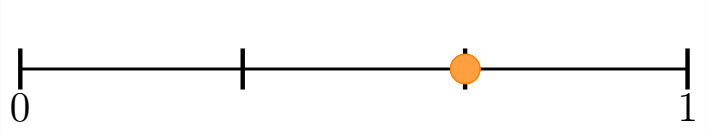
\includegraphics[width=165px]{../images/recta_num_frac2|3.png} \fillin[\fbox{$\dfrac{2}{3}$}][0in]
				\part 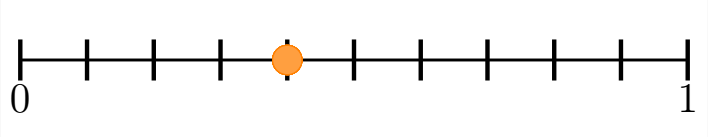
\includegraphics[width=165px]{../images/recta_num_frac4|10.png} \fillin[\fbox{$\dfrac{4}{10}$}][0in]
				\part 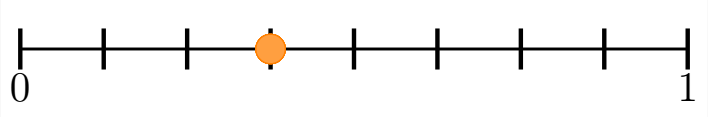
\includegraphics[width=165px]{../images/recta_num_frac3|8.png} \fillin[\fbox{$\dfrac{3}{8}$}][0in]
				\part 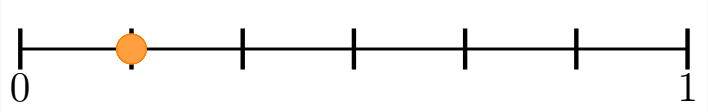
\includegraphics[width=165px]{../images/recta_num_frac1|6.png} \fillin[\fbox{$\dfrac{1}{6}$}][0in]
				\part 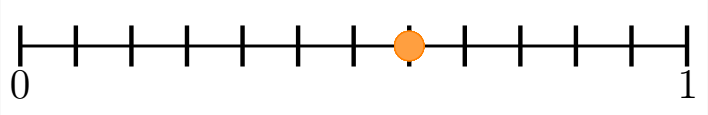
\includegraphics[width=165px]{../images/recta_num_frac7|12.png} \fillin[\fbox{$\dfrac{7}{12}$}][0in]
				\part 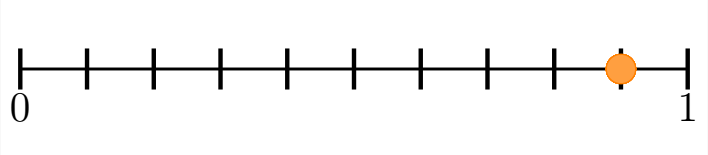
\includegraphics[width=165px]{../images/recta_num_frac9|10.png} \fillin[\fbox{$\dfrac{9}{10}$}][0in]
				\part 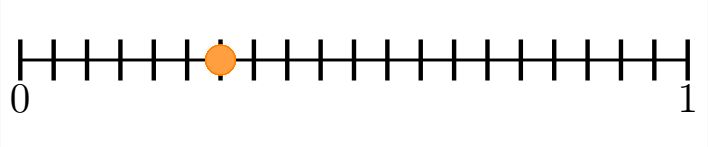
\includegraphics[width=165px]{../images/recta_num_frac6|20.png} \fillin[\fbox{$1\dfrac{6}{20}$}][0in]
				\part 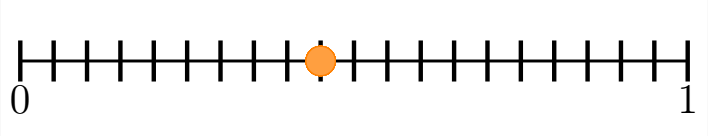
\includegraphics[width=165px]{../images/recta_num_frac9|20.png} \fillin[\fbox{$1\dfrac{9}{20}$}][0in]
				\part 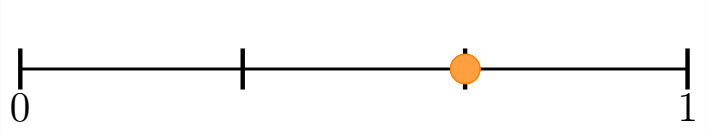
\includegraphics[width=165px]{../images/recta_num_frac2|3.png} \fillin[\fbox{$\dfrac{2}{3}$}][0in]
				\part 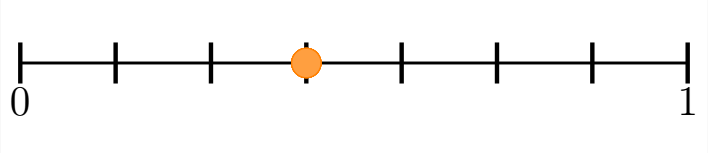
\includegraphics[width=165px]{../images/recta_num_frac3|7.png} \fillin[\fbox{$\dfrac{3}{7}$}][0in]
			\end{parts}
		\end{multicols}
	}

	% \subsection*{\ifprintanswers{Nombre de fracciones                       }\else{}\fi}

	\questionboxed[2]{Escribe la fracción que corresponda en cada inciso:

		\begin{parts}
			\part ¿Cómo se escribe numéricamente la fracción \textbf{siete catorceavos}?    \fillin[$\dfrac{7}{14}$][0in]
			\part ¿Cómo se escribe numéricamente la fracción \textbf{ocho onceavos}?   \fillin[$\dfrac{8}{11}$][0in]
			\part ¿Cómo se escribe numéricamente la fracción \textbf{doce séptimos}?    \fillin[$\dfrac{12}{7}$][0in]
			\part ¿Cómo se escribe numéricamente la fracción \textbf{nueve treceavos}?     \fillin[$\dfrac{9}{13}$][0in]
		\end{parts}
	}

	% \subsection*{\ifprintanswers{Representación de fracciones}\else{}\fi}
	\questionboxed[2]{Escribe sobre la línea la fracción que representa cada imagen:

		\begin{multicols}{5}
			\begin{parts}
				\part 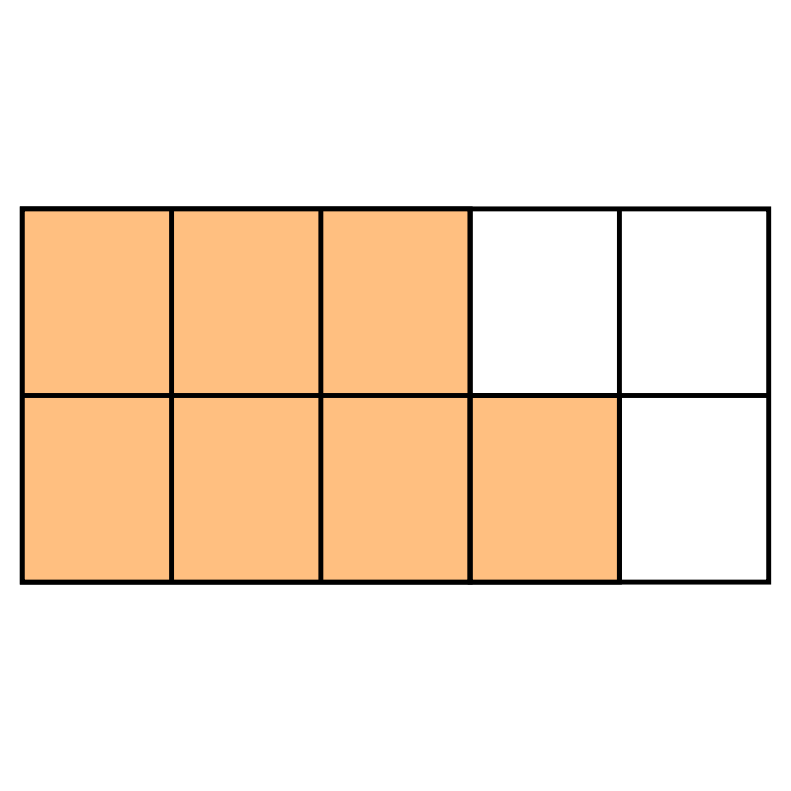
\includegraphics[width=45px]{../images/imagen_frac_5prim_7|10.png} \fillin[\fbox{$\dfrac{10}{20}$}][0in] \\[0.5em]
				\part 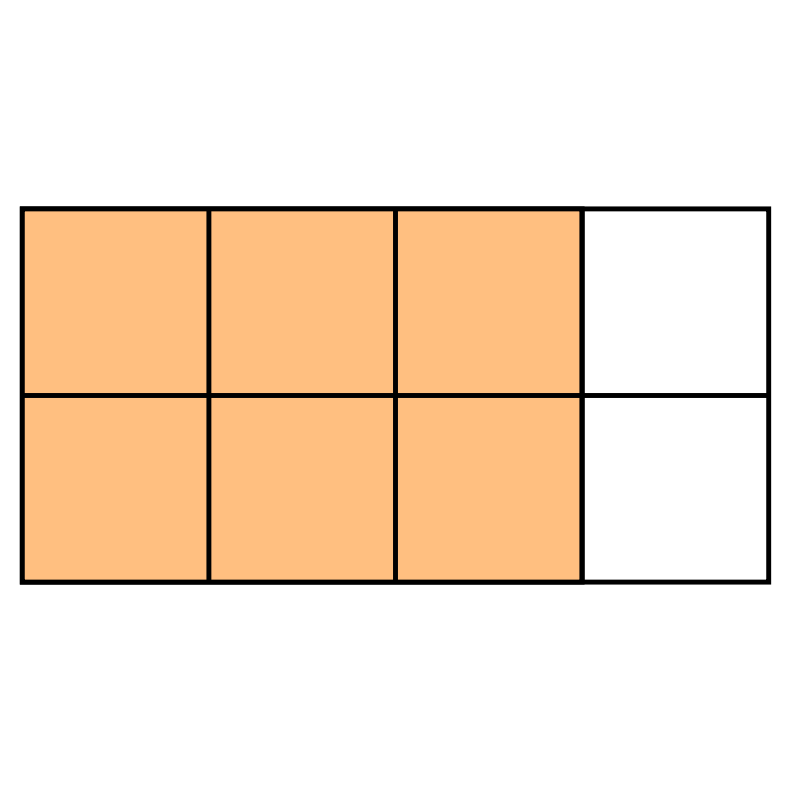
\includegraphics[width=45px]{../images/imagen_frac_5prim_6|8.png} \fillin[\fbox{$\dfrac{5}{6}$}][0in] \\[0.5em]
				\part 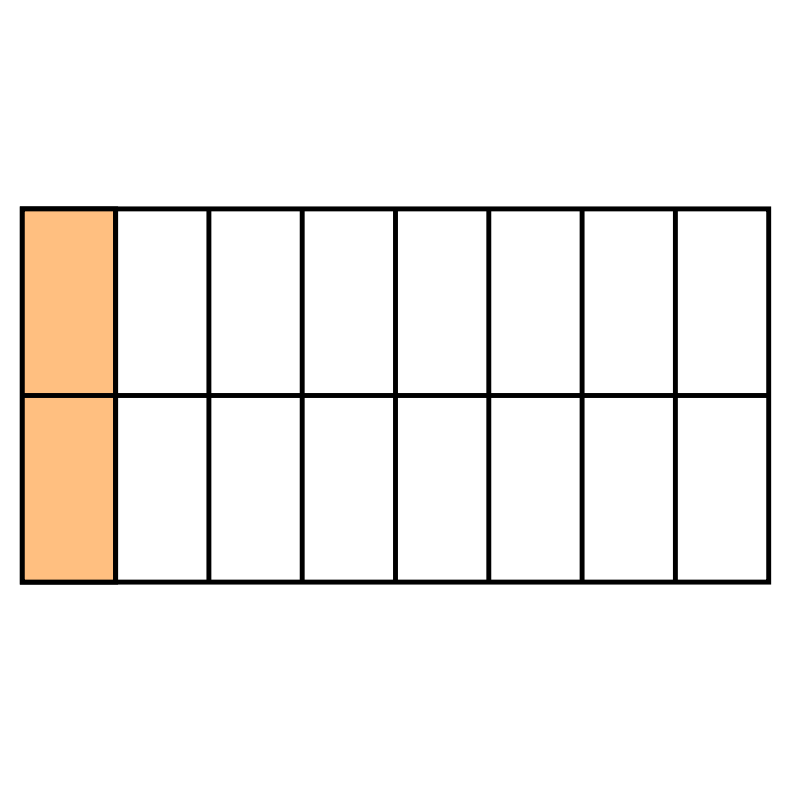
\includegraphics[width=45px]{../images/imagen_frac_5prim_2|16.png} \fillin[\fbox{$\dfrac{11}{16}$}][0in] \\[0.5em]
				\part 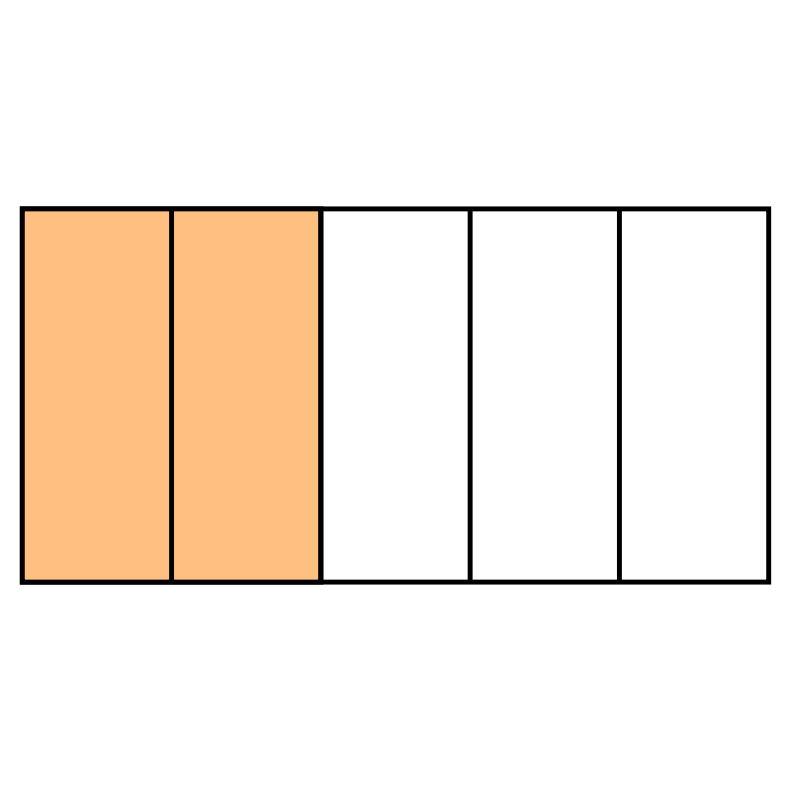
\includegraphics[width=45px]{../images/imagen_frac_5prim_2|5.png} \fillin[\fbox{$\dfrac{14}{16}$}][0in] \\[0.5em]
				\part 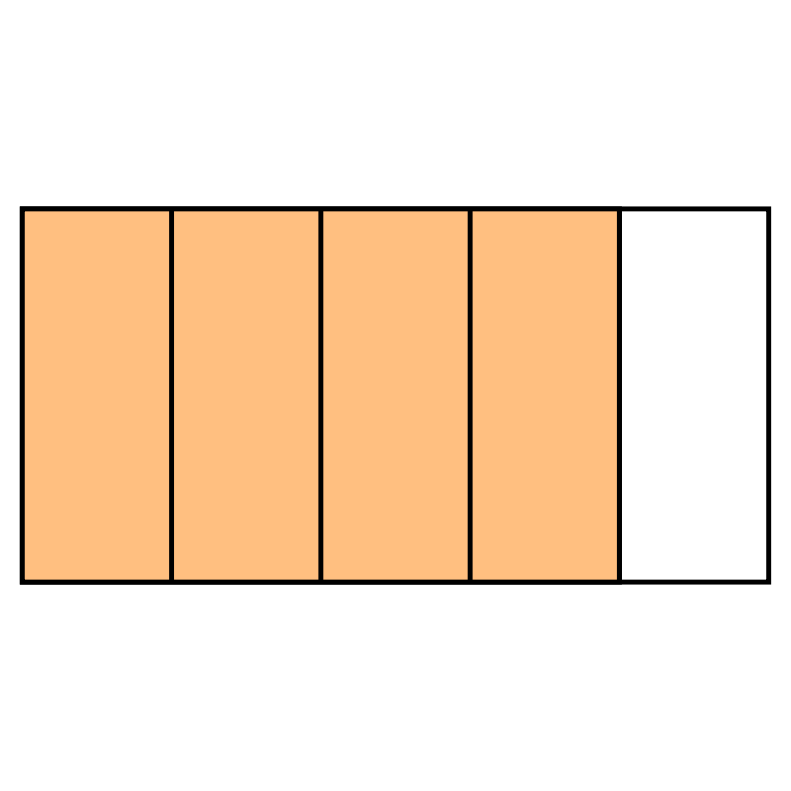
\includegraphics[width=45px]{../images/imagen_frac_5prim_4|5.png} \fillin[\fbox{$\dfrac{17}{20}$}][0in] \\[0.5em]
				\part 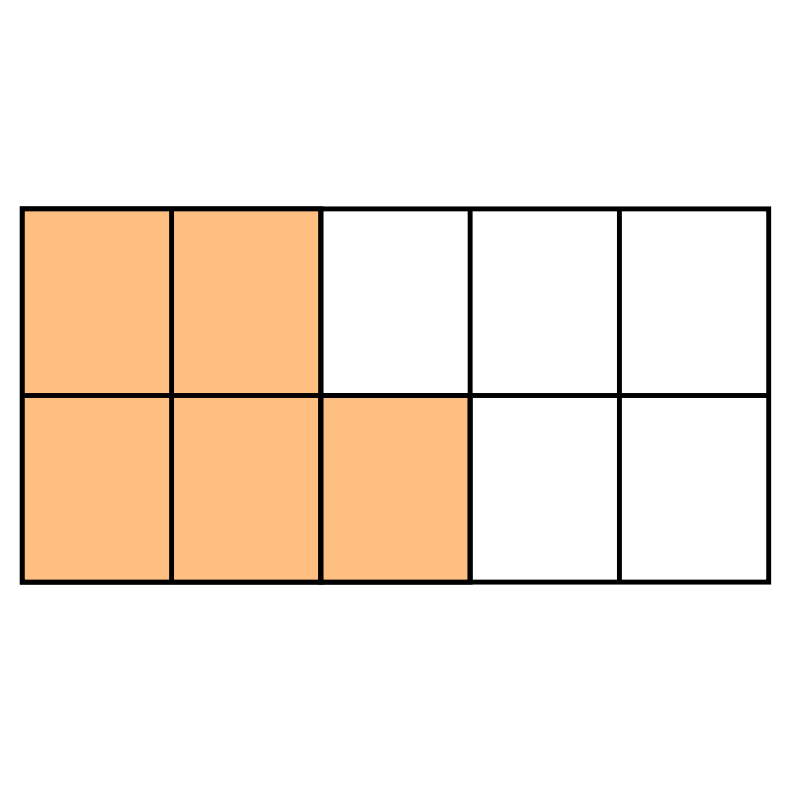
\includegraphics[width=45px]{../images/imagen_frac_5prim_5|10.png} \fillin[\fbox{$\dfrac{9}{16}$}][0in] \\[0.5em]
				\part 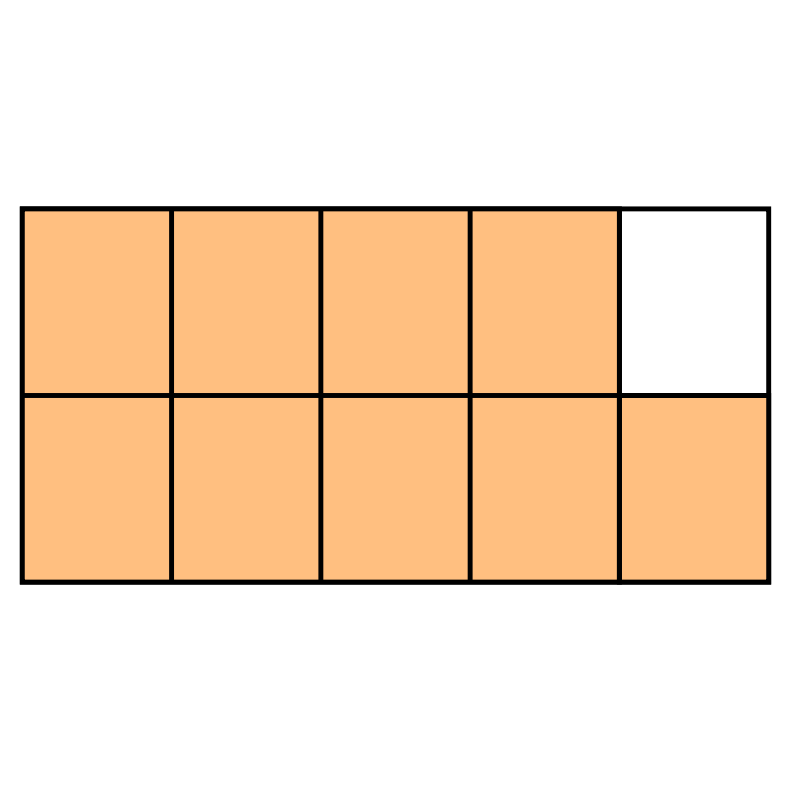
\includegraphics[width=45px]{../images/imagen_frac_5prim_9|10.png} \fillin[\fbox{$\dfrac{15}{20}$}][0in] \\[0.5em]
				\part 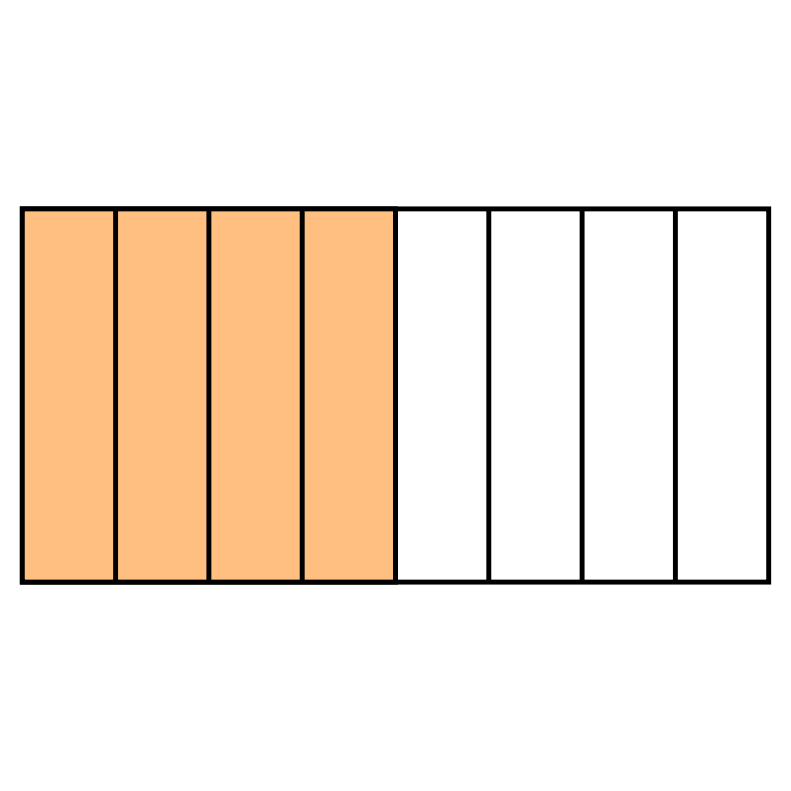
\includegraphics[width=45px]{../images/imagen_frac_5prim_4|8.png} \fillin[\fbox{$\dfrac{7}{8}$}][0in] \\[0.5em]
				\part 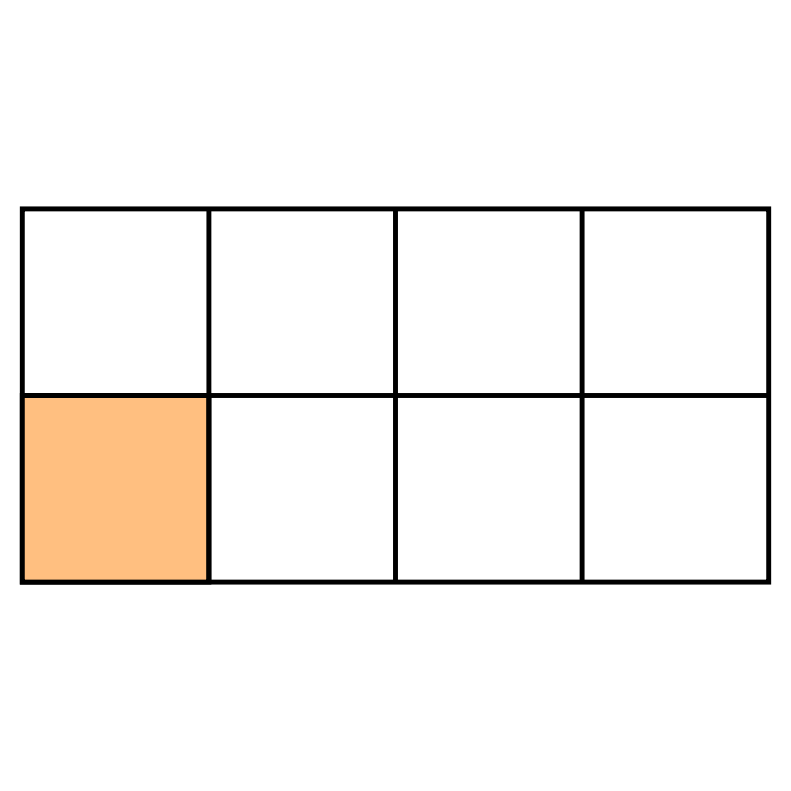
\includegraphics[width=45px]{../images/imagen_frac_5prim_1|8.png} \fillin[\fbox{$\dfrac{13}{20}$}][0in] \\[0.5em]
				\part 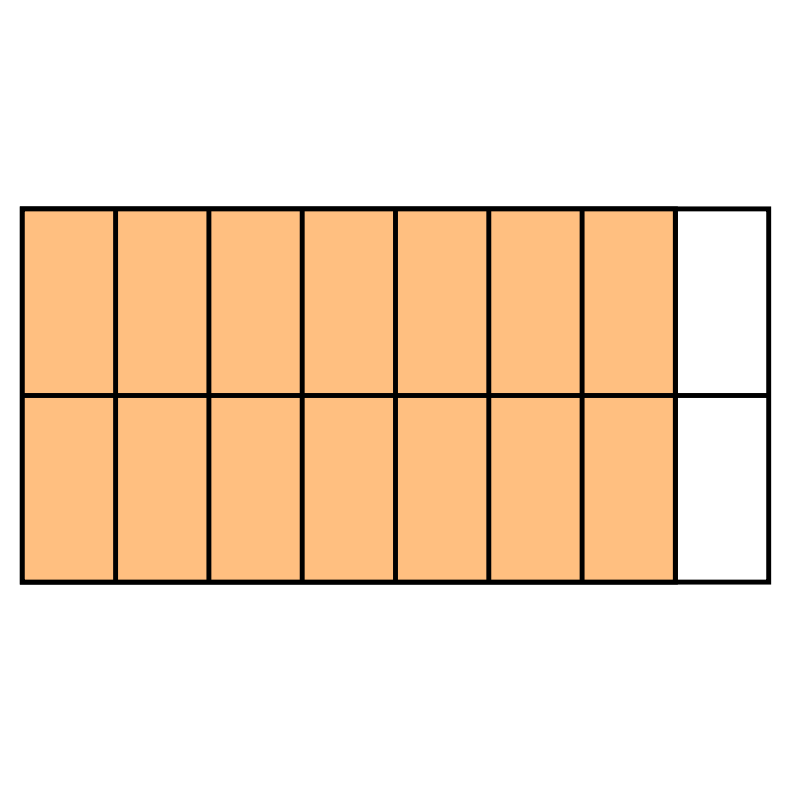
\includegraphics[width=45px]{../images/imagen_frac_5prim_14|16.png} \fillin[\fbox{$\dfrac{1}{20}$}][0in] \\[0.5em]
			\end{parts}
		\end{multicols}
	}






	% \subsection*{\ifprintanswers{Conversión de fracciones}
	\questionboxed[4]{Convierte la siguientes fracciones mixtas a impropias y viseversa:

		\begin{multicols}{3}
			\begin{parts}
				\part $4\dfrac{2}{3}= $  \fillin[$\dfrac{14}{3}$][0in]\\[0.5em]
				\part $\dfrac{13}{3}= $  \fillin[$4\dfrac{1}{3}$][0in]\\[0.5em]
				\part $2\dfrac{3}{10}= $ \fillin[$\dfrac{23}{10}$][0in]\\[0.5em]
				\part $\dfrac{43}{10}= $ \fillin[$4\dfrac{3}{10}$][0in]\\[0.5em]
				\part $5\dfrac{1}{5}= $  \fillin[$\dfrac{26}{5}$][0in]\\[0.5em]
				\part $\dfrac{51}{5}= $  \fillin[$10\dfrac{1}{5}$][0in]\\[0.5em]
			\end{parts}
		\end{multicols}
	}



	\addcontentsline{toc}{subsection}{Suma y resta de fracciones}
	\subsection*{Suma y resta de fracciones}
	% \subsection*{\ifprintanswers{Simplificación de fracciones          }
	% \subsection*{\ifprintanswers{Suma y resta con denominadores iguales}
	% \subsection*{\ifprintanswers{Suma con denominadores diferentes     }
	% \subsection*{\ifprintanswers{Resta con denominadores diferentes    }
	% \subsection*{\ifprintanswers{Sumas y restas con fracciones mixtas  }

	\questionboxed[15]{Realiza las siguientes operaciones de suma y resta de fracciones:

		\begin{multicols}{3}
			\begin{parts}
				\part $\dfrac{3}{10}+\dfrac{4}{5}=$ \fillin[$\dfrac{11}{10} = 1\dfrac{1}{10}$][0in] \\
				\part $\dfrac{3}{4}-\dfrac{2}{5}=$ \fillin[$\dfrac{7}{20}$][0in] \\
				\part $\dfrac{2}{3}-\dfrac{2}{5}=$ \fillin[$\dfrac{4}{15}$][0in] \\
				\part $\dfrac{3}{8}+\dfrac{7}{10}=$ \fillin[$\dfrac{43}{40} = 1\dfrac{3}{40}$][0in] \\
				% \part $\dfrac{3}{5}\times\dfrac{2}{3}=$ \fillin[$\dfrac{6}{15}$][0in]   \\
				% \part $\dfrac{7}{8}\times\dfrac{3}{4}=$ \fillin[$\dfrac{21}{32}$][0in] \\
				% \part $\dfrac{3}{5} \divisionsymbol\dfrac{2}{3}=$ \fillin[$\dfrac{9}{10}$][0in] \\
				% \part $\dfrac{7}{8} \divisionsymbol\dfrac{3}{4}=$ \fillin[$\dfrac{28}{24}$][0in]	\\
				\part $1\dfrac{1}{8}+1\dfrac{7}{8}=$ \fillin[$2\dfrac{8}{8} = 3$][0in] \\
			\end{parts}
		\end{multicols}
	}


	\addcontentsline{toc}{subsection}{Multiplicación y división de fracciones}
	\subsection*{Multiplicación y división de fracciones}
	% \subsection*{\ifprintanswers{Multiplicación de fracciones          }
	% \subsection*{\ifprintanswers{División de fracciones                }
	% \subsection*{\ifprintanswers{Multiplicación y división con enteros }
	% \subsection*{\ifprintanswers{Multiplicación con fracciones mixtas  }
	% \subsection*{\ifprintanswers{División con fracciones mixtas        }
	\questionboxed[15]{Realiza las siguientes operaciones de multiplicación y división de fracciones:

		\begin{multicols}{3}
			\begin{parts}
				% \part $\dfrac{3}{10}+\dfrac{4}{5}=$ \fillin[$\dfrac{11}{10} = 1\dfrac{1}{10}$][0in] \\
				% \part $\dfrac{3}{4}-\dfrac{2}{5}=$ \fillin[$\dfrac{7}{20}$][0in] \\
				% \part $\dfrac{2}{3}-\dfrac{2}{5}=$ \fillin[$\dfrac{4}{15}$][0in] \\
				% \part $\dfrac{3}{8}+\dfrac{7}{10}=$ \fillin[$\dfrac{43}{40} = 1\dfrac{3}{40}$][0in] \\
				\part $\dfrac{3}{5}\times\dfrac{2}{3}=$ \fillin[$\dfrac{6}{15}$][0in]   \\
				\part $\dfrac{7}{8}\times\dfrac{3}{4}=$ \fillin[$\dfrac{21}{32}$][0in] \\
				\part $\dfrac{3}{5} \divisionsymbol\dfrac{2}{3}=$ \fillin[$\dfrac{9}{10}$][0in] \\
				\part $\dfrac{7}{8} \divisionsymbol\dfrac{3}{4}=$ \fillin[$\dfrac{28}{24}$][0in]	\\
				% \part $1\dfrac{1}{8}+1\dfrac{7}{8}=$ \fillin[$2\dfrac{8}{8} = 3$][0in] \\
			\end{parts}
		\end{multicols}
	}


	\addcontentsline{toc}{subsection}{MCD y MCM}
	\subsection*{MCD y MCM}
	% \subsection*{\ifprintanswers{Factores primos                       }
	% \subsection*{\ifprintanswers{Fracciones equivalentes               }
	% \subsection*{\ifprintanswers{Mínimo común múltiplo                 }
	% \subsection*{\ifprintanswers{Máximo común divisor                  }
	% \subsection*{\ifprintanswers{Simplificación de fracciones          }
	\addcontentsline{toc}{subsection}{Decimales y porcentajes}
	\subsection*{Decimales y porcentajes}
	% \subsection*{\ifprintanswers{Decimales en la recta númerica        }
	% \subsection*{\ifprintanswers{Porcentaje como decimales             }
	% \subsection*{\ifprintanswers{Porcentaje de números                 }
	% \subsection*{\ifprintanswers{Conversión de decimales a fracciones  }
	% \subsection*{\ifprintanswers{Conversión de fracciones a decimales  }  

	\addcontentsline{toc}{section}{Unidad 3}
	\section*{Unidad 3}
	\addcontentsline{toc}{subsection}{Estadística y gráficas}
	\subsection*{Estadística y gráficas}
	% \subsection*{\ifprintanswers{Mediana    }                                            
	% \subsection*{\ifprintanswers{Moda       }                                            
	% \subsection*{\ifprintanswers{Media      }
	% \subsection*{\ifprintanswers{Interpretación de gráficas         }
	% \subsection*{\ifprintanswers{Tablas de variación                }
	\addcontentsline{toc}{subsection}{Círculo}
	\subsection*{Círculo}
	% \subsection*{\ifprintanswers{Diámetro de un círculo             }
	% \subsection*{\ifprintanswers{Radio de un círculo                }
	% \subsection*{\ifprintanswers{Perímetro de un círculo            }
	% \subsection*{\ifprintanswers{Área de un círculo                 }
	% \subsection*{\ifprintanswers{Líneas del círculo                 }
	\addcontentsline{toc}{subsection}{Figuras geométricas}
	\subsection*{Figuras geométricas}

	% \subsection*{\ifprintanswers{Nombre de figuras                  }
	\questionboxed[2]{Escribe sobre la línea el nombre que recibe cada figura geométrica de acuerdo con su número de lados:

		\begin{multicols}{3}
			\begin{parts}
				\part 
\includegraphics[width=75px]{../images/pentagono_azul.png}  \fillin[pentágono][0.75in]
				\part 
\includegraphics[width=75px]{../images/nonagono_azul.png}   \fillin[nonágono][0.75in]
				\part 
\includegraphics[width=75px]{../images/decagono_azul.png}   \fillin[decágono][0.75in]
				\part 
\includegraphics[width=75px]{../images/hexagono_azul.png}   \fillin[hexágono][0.75in]
				\part 
\includegraphics[width=75px]{../images/rectangulo_azul.png} \fillin[rectángulo][0.75in]
				\part 
\includegraphics[width=75px]{../images/cuadrado_azul.png}   \fillin[cuadrado][0.75in]
			\end{parts}
		\end{multicols}
	}


	% \subsection*{\ifprintanswers{Elementos de figuras               }
	% \subsection*{\ifprintanswers{Perímetro  }
	\questionboxed[4]{Contesta las preguntas sobre perímetros de figuras geométricas

		\begin{multicols}{2}
			\begin{parts}
				\part ¿Cuál es el perímetro de un rectángulo cuya base mide 38 y su altura mide 19?

				\begin{solutionbox}{1cm}
					\[P=38+19+38+19=\color{red}114\]
				\end{solutionbox}

				\part ¿Cuál es el perímetro de un cuadrado que sus lados miden 5?

				\begin{solutionbox}{1cm}
					\[P=5+5+5+5=\color{red}20\]
				\end{solutionbox}

				\part ¿Cuál es el perímetro de un pentágono que sus lados miden 18?

				\begin{solutionbox}{1cm}
					\[P=18 \times 5=\color{red}90\]
				\end{solutionbox}

				% \part ¿Cuál es el perímetro de un octágono que sus lados miden 15?

				% \begin{solutionbox}{1cm}
				% 	\[P=15 \times 8=\color{red}120\]
				% \end{solutionbox}

				\part ¿Cuál es el perímetro de un rombo que sus lados miden 16?

				\begin{solutionbox}{1cm}
					\[P=16 \times 4=\color{red}64\]
				\end{solutionbox}

			\end{parts}
		\end{multicols}
	}

	% \subsection*{\ifprintanswers{Área       }
	\questionboxed[4]{Contesta las preguntas sobre áreas de figuras geométricas

		\begin{multicols}{2}
			\begin{parts}
				\part ¿Cuál es el área de un triángulo cuya base mide 18 y su altura mide 11?

				\begin{solutionbox}{1.5cm}
					\[A=\dfrac{18 \times 11}{2}=\color{red}99\]
				\end{solutionbox}

				\part ¿Cuál es el área de un cuadrado que sus lados miden 29?

				\begin{solutionbox}{1.5cm}
					\[A=29 \times 29=\color{red}841\]
				\end{solutionbox}
			\end{parts}
		\end{multicols}
	}

	% \subsection*{\ifprintanswers{Resolución de problemas            }
	\addcontentsline{toc}{subsection}{Resolución de problemas}
	\subsection*{Resolución de problemas}
	% \subsection*{\ifprintanswers{Unidades de tiempo y reloj         }
	% \subsection*{\ifprintanswers{Cuerpos geométricos 1              }
	% \subsection*{\ifprintanswers{Cuerpos geométricos 2              }
	% \subsection*{\ifprintanswers{Resolución de problemas 1          }
	% \subsection*{\ifprintanswers{Resolución de problemas 2          }
	\addcontentsline{toc}{subsection}{Sistema de unidades}
	\subsection*{Sistema de unidades}
	% \subsection*{\ifprintanswers{Multiplicaciones por múltiplos de 10}
	% \subsection*{\ifprintanswers{Divisiones por múltiplos de 10     }
	% \subsection*{\ifprintanswers{Unidades de longitud               }
	% \subsection*{\ifprintanswers{Unidades de masa                   }
	% \subsection*{\ifprintanswers{Unidades de capacidad              }
	\questionboxed[3]{Realiza las siguientes operaciones:

		\begin{multicols}{3}
			\begin{parts}
				\part $ 55 \times 10000=$   \fillin[550000][0.5in]
				\part $ 135 \times 100=$   \fillin[13500][0.5in]
				\part $ 369 \times 10000=$   \fillin[3690000][0.5in]
				\part $ 88 \times 10=$   \fillin[880][0.5in]
				\part $ 1215 \times 100=$   \fillin[121500][0.5in]
				\part $ 300 \times 10000=$   \fillin[3000000][0.5in]
				\part $ 224 \times 1000=$   \fillin[224000][0.5in]
				\part $ 13 \times 1000=$   \fillin[13000][0.5in]
				\part $ 134 \times 100000=$   \fillin[13400000][0.5in]
				\part $ 188 \times 10=$   \fillin[1880][0.5in]
				\part $ 401 \times 1000=$   \fillin[401000][0.5in]
				\part $ 42 \times 10=$   \fillin[420][0.5in]
				\part $ 92 \times 1000=$   \fillin[92000][0.5in]
				\part $ 1050 \times 1000=$   \fillin[1050000][0.5in]
				\part $ 19 \times 100=$   \fillin[1900][0.5in]
			\end{parts}
		\end{multicols}
	}




	\questionboxed[3]{Realiza las siguientes conversiones de unidades de longitud:

		\begin{multicols}{2}
			\begin{parts}
				\part De 157 kilómetros a hectómetros. \\ \fillin[1570][0.6in] hm
				\part De 25 centímetros a milímetros.  \\ \fillin[250][0.6in] mm
				\part De 27 kilómetros a decámetros.   \\ \fillin[2700][0.6in] Dm
				\part De 17 kilómetros a hectómetros.  \\ \fillin[170][0.6in] hm
				\part De 69 kilómetros a centímetros.  \\ \fillin[6900000][0.6in] cm
				\part De 59 decímetros a centímetros.  \\ \fillin[590][0.6in] cm
				\part De 26 metros a decímetros.       \\ \fillin[260][0.6in] dm
				\part De 4 kilómetros a milímetros.    \\ \fillin[4000000][0.6in] mm
				\part De 135 kilómetros a decámetros.  \\ \fillin[13500][0.6in] Dm
				\part De 112 kilómetros a hectómetros. \\ \fillin[1120][0.6in] hm
			\end{parts}
		\end{multicols}
	}


	% \subsection*{\ifprintanswers{Unidades de masa 	                          }\else{}\fi}
	\questionboxed[3]{Realiza las siguientes conversiones de unidades de longitud:

		\begin{multicols}{2}
			\begin{parts}
				\part De 205 gramos a decigramos    \hfill \fillin[2050][0.5in] dg
				\part De 25 kilogramos a gramos     \hfill \fillin[25000][0.5in] g
				\part De 58 kilogramos a gramos     \hfill \fillin[58000][0.5in] g
				\part De 45 decagramos a gramos     \hfill \fillin[450][0.5in] g
				\part De 134 gramos a decigramos    \hfill \fillin[1340][0.5in] dg
				\part De 282 gramos a miligramos    \hfill \fillin[282000][0.5in] mg
				\part De 117 decagramos a gramos    \hfill \fillin[1170][0.5in] g
				\part De 17 decigramos a miligramos \hfill \fillin[1700][0.5in] mg
				\part De 115 gramos a centigramos   \hfill \fillin[11500][0.5in] cg
				\part De 62 gramos a miligramos     \hfill \fillin[62000][0.5in] mg
			\end{parts}
		\end{multicols}
	}
\end{questions}
\end{document}